\documentclass[compress,red,mathsans,10pt]{beamer}
%\documentclass[handout, compress,red,mathsans,10pt]{beamer}
\usepackage{beamerthemesplit}
\usepackage{amssymb}
%\usetheme{Antibes}
%\usepackage{pgf,pgfarrows,pgfnodes}
\usepackage[catalan]{babel}
%\usepackage[latin1]{inputenc}
\usepackage[utf8]{inputenc}
%\usepackage[pdftex]{graphicx}

\setbeamercolor{uppercol}{fg=white,bg=purple}%
\setbeamercolor{lowercol}{fg=black,bg=pink}%


\usecolortheme{lily}
\begin{document}
\title{Fonaments i Aplicacions de Processament Digital dels Senyal}
\subtitle{Grau Telem\`atica. Curs 2012/13}  
\author{Jos\'e Luis Lisani}
\date{}



\frame{\titlepage} 

%\frame{\frametitle{Table of contents}\tableofcontents} 

\section{Presentaci\'o} 
\frame{\frametitle{Informaci\'o general}	
\begin{itemize}
\item Professor: Jos\'e Luis Lisani
\item [] Despatx: Anselm Turmeda D-239
\item [] E-mail: joseluis.lisani@uib.es
\item Horari:
	\begin{center}
	\begin{tabular}{|l|c|} \hline
	Dia & Hora \\ \hline
	Dilluns & 15:30 -- 17:30 
       \\ \hline
	Dimecres & 17:30 -- 18:30 \\ 
                   & (18:30-19h30  \qquad 3 sessions pr\`actiques)
                   \\ \hline
	\end{tabular}
	\end{center}
\item Documentaci\'o:
	\begin{itemize}
	\item campus extens (apunts, llistes problemes, anuncis)
	\item UIB digital (guia docent, cronograma)
	\end{itemize} 
\item Tutories:
\begin{itemize}
\item dimarts 11h30-13h,  dijous 11h30-13h
\end{itemize}
\item[] <2-> \color{red}Concertar previament per email\color{black}
\end{itemize}
}


\frame{\frametitle{Temari}
\begin{itemize}
\item Tema 1.Introducci\'o.
\item Tema 2. Senyals i sistemes.
	\item [] <2->\color{red}Control:  20/03\color{black}
\item Tema 3. Transformada Z.
	\item [] <2-> \color{red}Control:  17/04\color{black}
\item Tema 4. Transformada de Fourier discreta. Mostreig.
	\item [] <2->\color{red}Control:   22/05\color{black}
\item Tema 5. Filtres digitals.
	\item [] <2->\color{red}Entrega pr\`actica ordinador: 24/06\color{black}
\end{itemize}
}

\frame{\frametitle{Calendari}
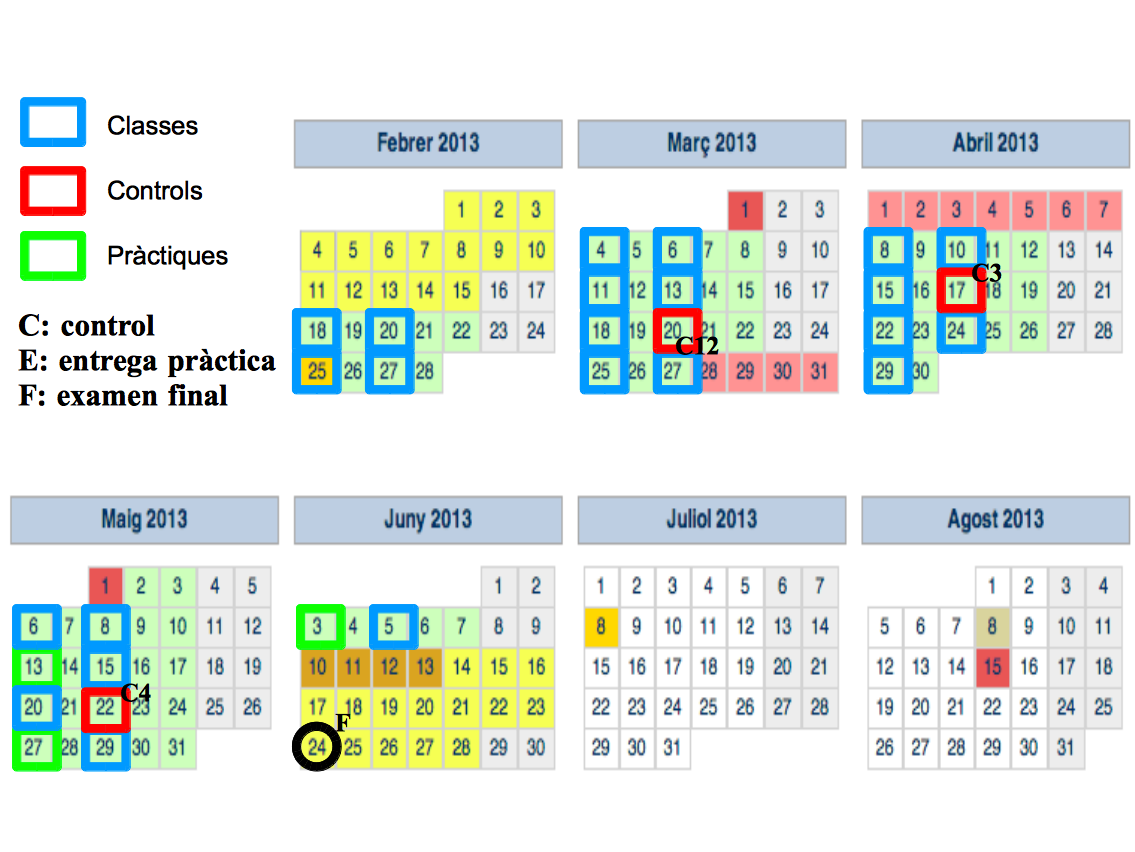
\includegraphics[width=11cm]{calendari2Sb.png}
}

\frame{\frametitle{Material}
\begin{itemize}
\item Apunts
\item Llistes de problemes 
\item Enunciat de la pr\`actica
\item Enlla\c{c}os d'inter\'es
\item[]
\item[] <2-> \color{red} Disponible a Campus Extens \color{black}
\end{itemize}
}

\frame{\frametitle{Avaluaci\'o}
\begin{itemize}
\item Activitats d'avaluaci\'o:
\begin{itemize}
\item Avaluaci\'o cont\'inua:
\begin{itemize}
\item Controls: 20/03 (temes 1 i 2), 17/04 (tema 3), 22/05 (tema 4) 
	\item[] <2-> \color{red}Dates flexibles per a la gent que fa feina\color{black} 
\item Pr\`actica ordinador: 24/06 (tema 5)
\end{itemize}
\item Examen final: 24/06 (tot), \color{red}11/09 (tot)\color{black}
\end{itemize}
	\item <3-> Criteris d'avaluaci\'o:
	\begin{itemize}
	\item Nota m\'inima de l'examen final: 3
	\item Les notes de l'avaluaci\'o cont\'inua (controls i pr\`actica) es guarden fins el setembre.
	\item Els controls no s\'on recuperables. La pr\`actica d'ordinador es pot recuperar per setembre.
	\item Nota final = $30\%$ nota mitjana controls + $20\%$ nota pr\`actica  + $50\%$ nota examen final
	\end{itemize}
\end{itemize}
}


\end{document}